\chapter{Two Example Measurements}
\label{standards}
A successful measurement of a reaction in inverse kinematics requires a high-efficiency, high-resolution detector system with large acceptance and good background suppression.  The traditional solution to these issues is to use a large detector array with fine angular resolution~\cite{Pollacco_2005,Catford_2005,Demonchy_2007,Kanungo_2010}.  This chapter discusses two benchmark reaction measurements in inverse kinematics using the traditional---or non-solenoidal---detector approach wherein the laboratory energy $E_\mathrm{lab}$ of the detected particles is measured as a function of the laboratory angle $\theta_\mathrm{lab}$ to determine the center-of-mass quantities.

\section[\texorpdfstring{The $^\text{12}$B\lowercase{($d$,$p$)} Measurement}{The 12B(d,p) Measurement}]{\texorpdfstring{The $^\mathbf{12}$B($d$,$p$) Measurement}{The 12B(d,p) Measurement}}
\subsection{Introduction}
\label{b12intro}
A measurement of the $^{12}$B($d$,$p$) reaction was carried out at Argonne National Laboratory to study the neutron-rich $N=8$ nucleus $^{13}$B.  The details of this measurement are described in Ref.~\cite{Lee_2010}; this section summarizes those results.  Originally, the main purpose of this experiment was a nuclear structure study.  There is a pair of excited states in $^{13}$B near 3.6\,MeV, separated by 199\,keV, which had (at the time of the experiment) unknown spins. % and parities.
  The aim of this measurement was to resolve this doublet and through the analysis of the resulting angular distributions, determine the angular momentum transfer $\ell_n$ and assign spins and parities $J^\pi$ to the states.

\subsection{Experimental Setup}
%\section{Ludwig's Castle}
The experiment was carried out in the scattering chamber upstream from the Enge Split-Pole Spectrograph in ATLAS Target Area III (SPSIII), referred to internally as Ludwig's Castle.  
\subsubsection{Beam Production}
\label{beamprod}
$^{12}$B is unstable against $\beta$-decay with a half-life of $T_{1/2}=20.2$\,ms.  Therefore, a reaction involving $^{12}$B must be performed in inverse kinematics.  In this example, the $^{12}$B beam is produced in-flight, following the method %of beam production used in this experiment
which is described in detail in Ref.~\cite{Harss_2000}.  A primary beam of stable $^{11}$B ions at an energy of 81\,MeV and an intensity of 100\,pnA bombarded a cryogenic gas cell to produce the secondary radioactive beam. % via the $d$($^{12}$B,$p$) reaction.
The production cell is shown in Fig.~\ref{gas_cell}.  The gas cell was filled with D$_2$ deuterium gas at a pressure of 1400\,mbar and temperature of $-185$\,$^\circ$C to produce a target with an areal density of 1.6\,mg/cm$^2$.  The secondary $^{12}$B beam was produced in the neutron transfer reaction $d$($^{11}$B,$^{12}$B)$p$.  The resulting radioactive beam bombarded an 150\,$\mu$g/cm$^2$ target of deuterated polyethylene (C$_2$D$_4$)$_n$ with an average beam intensity of $1.2\times 10^5$\,ions/s.

\begin{figure}%
\centering
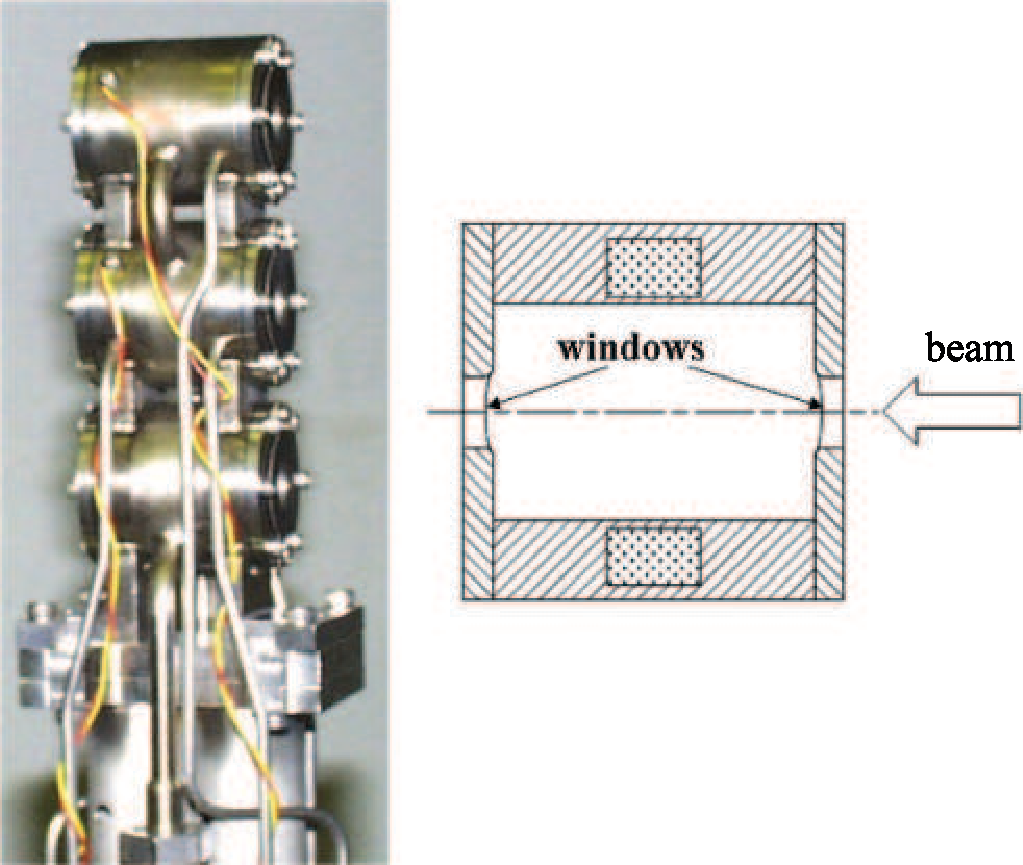
\includegraphics[height=0.5\textwidth,width=\columnwidth,keepaspectratio]{GastargetFig2}%
\caption[Gas cell used for in-flight beam production at ATLAS]{Gas cell used for in-flight beam production at ATLAS.  The type of gas cell used to produce the radioactive $^{12}$B beam in-flight are 3.7\,cm long and 2.54\,cm in diameter. Havar$\textsuperscript{\textregistered}$ foils 1.9\,mg/cm$^2$ thick serve as windows on the entrance and exit of the gas cell.}
\label{gas_cell}%
\end{figure}

\subsubsection{Detectors}
The  detector setup for measuring transfer reactions within Ludwig's Castle is described in Ref.~\cite{Wuosmaa_2005}.  The same basic setup was used in this measurement.  The detector array utilized in this experiment consists of three 500\,$\mu$m thick double-sided silicon strip detectors (DSSD) of design S1 manufactured by Micron Semiconductor.  The annular detectors have an inner radius of 24\,mm and an outer radius of 48\,mm, for a total active area of 53\,cm$^2$.  One side of each detector is segmented into 16 concentric rings of $\Delta r=1.5$\,mm, while the other side is segmented into 16 wedges, each covering $\Delta \phi =22.5^\circ$; thus each detector requires 32 electronics channels.  To suppress spurious counts, a detector signal is required in an element on both sides of a given detector in order to be included in the trigger logic.  Heavy recoils are identified downstream from the target in a $\Delta E$-$E$ detector array discussed in Chapt.~\ref{recoil}.  In an adjacent scattering chamber downstream from the heavy recoil detectors, a surface barrier detector is placed in the beam path behind an % 100$\times$
 attenuator to monitor the beam current.

Fig.~\ref{annular_dets} shows the physical relationship of the detectors to the target foil within the scattering chamber.  The  $^{12}$B($d$,$p$) reaction has a $K_\mathrm{g.s.}$-value of 0.61, which means forward angles in the center-of-mass correspond to rearward angles in the laboratory ($\theta_\mathrm{lab}>90^\circ$); hence the detector array is position upstream from the target foil.  Table~\ref{coverage} shows the solid-angle coverage for the detector array.  The entire array covered a solid angle of 1.10\,sr.

\begin{figure}%
\centering
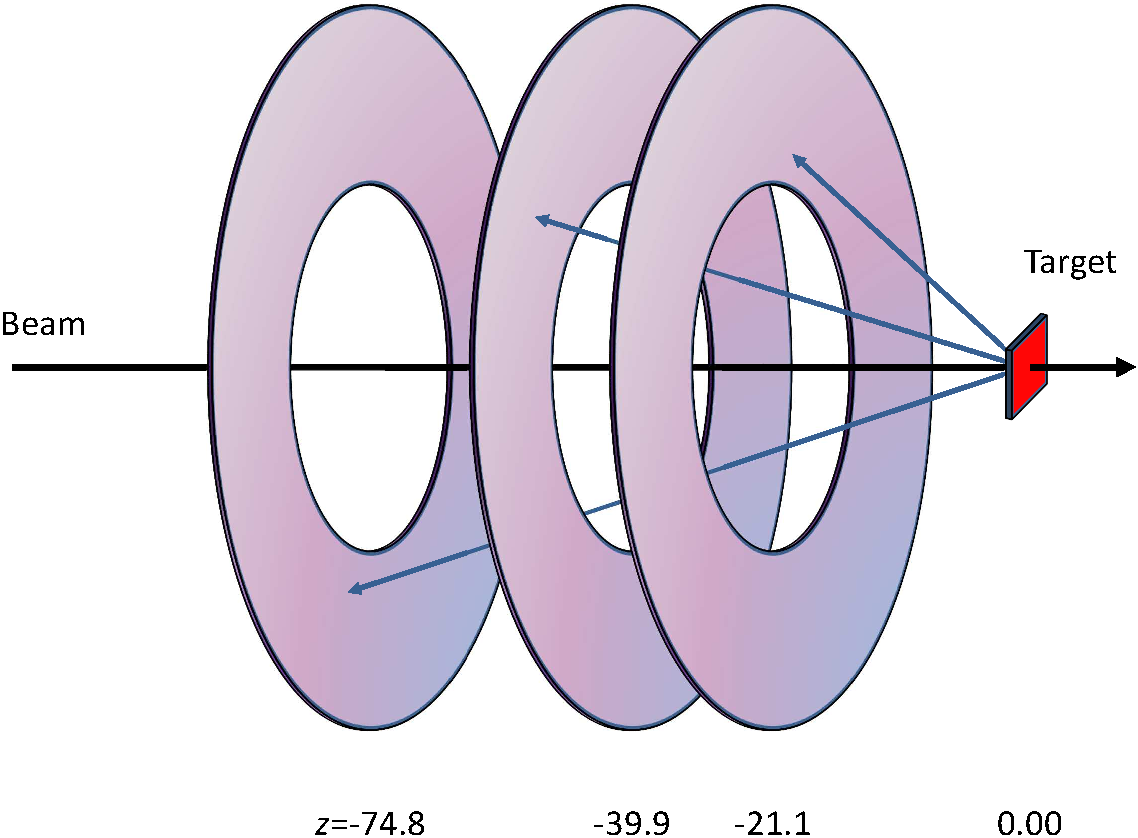
\includegraphics[width=\columnwidth,height=0.33\textheight,keepaspectratio]{annular}%
\caption[Detector setup for the $^{12}$B($d$,$p$) measurement in inverse kinematics]{Detector setup for the $^{12}$B($d$,$p$) measurement in inverse kinematics (drawn to scale).  Protons ejected in the rearward hemisphere ($\theta_\mathrm{lab}>90^\circ$) are detected by three annular detectors covering $114^\circ<\theta_\mathrm{lab}<162^\circ$.  }%
\label{annular_dets}%
\end{figure}

\begin{table}%
\centering
\begin{tabular}{ccrrcrrcc}
\hline
Det.&$z$&\multicolumn{2}{c}{$\theta_\mathrm{lab}$}&&\multicolumn{2}{c}{$\theta_\mathrm{cm}$}&$\Delta \cos(\theta_\mathrm{cm})$&$\Delta \Omega$\\ \cline{3-4} \cline{6-7}
&(mm)&\multicolumn{1}{c}{$\theta_1$}&\multicolumn{1}{c}{$\theta_2$}&&\multicolumn{1}{c}{$\theta_1$}&\multicolumn{1}{c}{$\theta_2$}&&(sr)\\
\hline \hline
1&$-21.1$&113.7&131.3&&32.4 &21.5 & 0.086  & 0.54\\
2&$-39.9$&121.9&141.2&&27.0 &16.4 & 0.068  & 0.43\\
3&$-74.8$&147.3&162.2&&13.5 &7.1 & 0.020  & 0.13\\
  \multicolumn{7}{r}{Total} &0.175&1.10\\
 \hline
\end{tabular}
\caption[Detector positions and solid angle coverage for the $^{12}$B($d$,$p$) measurement]{Detector positions and solid angle coverage for the $^{12}$B($d$,$p$) measurement.  Protons ejected in the rearward hemisphere ($\theta_\mathrm{lab}>90^\circ$) are detected by three annular detectors covering $114^\circ<\theta_\mathrm{lab}<162^\circ$.  }
\label{coverage}
\end{table}

\subsection{Results}
\begin{figure}%
\centering
\hspace*{\stretch{1}}%
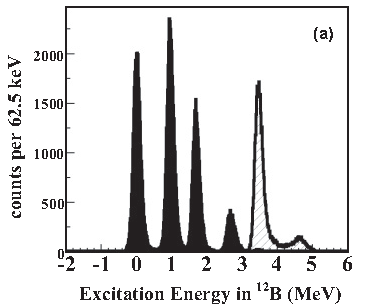
\includegraphics[width=0.45\textwidth,height=0.33\textheight,keepaspectratio]{Lee_2010_fig1b}\hspace*{\stretch{1}}
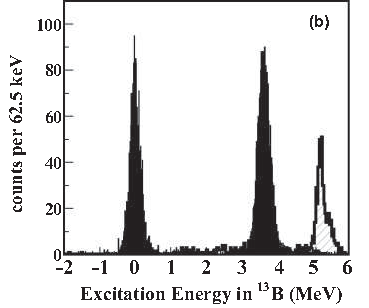
\includegraphics[width=0.45\textwidth,height=0.33\textheight,keepaspectratio]{Lee_2010_fig1d}\hspace*{\stretch{1}}
\caption[Excitation energy spectra from the $^{11,12}$B($d$,$p$) reactions in inverse kinematics]{Excitation energy spectra from the $^{11,12}$B($d$,$p$) reactions in inverse kinematics.  The energy resolution is 250\,keV.  The black peaks in both spectra correspond states populated in the residual nucleus which lie below the neutron-decay threshold; 3.4\,MeV for $^{12}$B and 4.9\,MeV for $^{13}$B.  The white (hatched) peaks correspond to states which are neutron-unbound.  (a) In the $^{11}$B($d$,$p$) spectrum, the $\Delta E_x=102$\,keV doublet near 2.7\,MeV is unresolved.  (b) In the $^{12}$B($d$,$p$) spectrum, the $\Delta E_x=199$\,keV doublet near 3.6\,MeV is unresolved.  Figure from Ref.~\cite[Fig.~1]{Lee_2010}.}
\label{b11b12_spec}%
\end{figure}

As shown in Table~\ref{error_prop}, the expected energy resolution of the $^{12}$B($d$,$p$) reaction is on the order of 120\,keV.  This estimate neglects beam spot size ($\approx 3$\,mm ) and target thickness (150\,$\mu$g/cm$^2$) effects. The beam spot size will have the same effect on any measurement.  The target thickness, however, has a pronounced effect on the $Q$-value resolution in inverse kinematics because the heavy ion experiences significant energy loss entering and exiting the target. %The beam spot size was 
Therefore, the reported $Q$-value resolution of 250\,keV is not surprising.  However, this resolution was insufficient to resolve the states at $E_x=3.482$ and 3.681\,MeV ($\Delta E_x=199$\,keV).  Therefore the separate angular distributions of these states could not be analyzed, making a determination of the angular momentum transfer impossible.  Fig.~\ref{b11b12_spec} shows the excitation energy spectra for both reactions.  The measurement of this reaction was re\-at\-tempt\-ed in order to separate these states using the HELIOS spectrometer as discussed in Chapt.~\ref{rib_com}.

Although %the $Q$-value resolution of this measurement was insufficient to separate the doublet near 3.6\,MeV, 
the original aim of this experiment was not realized,
the experiment did provide a new measurement that had astrophysical implications.  Eq.~\ref{eq:a12rproc} shows the $r$-process path through the light elements.  Included in the reaction chain is neutron capture on $^{11}$B (indicated by the underbrace).  The $^{11}$B($d$,$p$)$^{12}B$ neutron-transfer reaction is an example of a measurement that can be used to study the $r$-process.  Recoil tagging, using particle identification in the $\Delta E$-$E$ array (discussed in Chapt.~\ref{recoil}), was used to measure the branching ratio of $^{12}$B decay.  The neutron-unbound 3.389\,MeV state in $^{12}$B is predominately populated in coincidence with the recoiling $^{12}$B nucleus, corresponding to $\gamma$-decay of $^{12}$B$^\textrm{*}$.  However, a fraction of the events populating the 3.389\,MeV state were measured in coincidence with a $^{11}$B, corresponding to in-flight $n$-decay.   The ratio of the yield of these events is related to resonant neutron capture in $^{11}$B which contributes to both the overall rate of the $r$-process~\cite{Surman_2009}.  The details of this relationship are discussed in Ref.~\cite{Lee_2010}.

\begin{equation}
^{1}\textrm{H}(n,\gamma)^{2}\textrm{H}(n,\gamma)^{3}\textrm{H}(d,n)^{4}\textrm{He}(t,\gamma)^{7}\textrm{Li}(n,\gamma)^{8}\textrm{Li}(\alpha,n)\underbrace{^{11}\textrm{B}(n,\gamma)^{12}\textrm{B}}(\beta^-)^{12}\textrm{C}(n,\gamma)^{13}\textrm{C}
\label{eq:a12rproc}
\end{equation}


\section[\texorpdfstring{The $^\text{132}$S\lowercase{n($d$,$p$)} Measurement}{The 132Sn(d,p) Measurement}]{\texorpdfstring{The $^\mathbf{132}$Sn($d$,$p$) Measurement}{The 132Sn(d,p) Measurement}}
\subsection{Introduction}
%\section{ORRUBA}
A sophisticated example of a large acceptance array with excellent resolution is the Oak Ridge Rutgers university Barrel Array (ORRUBA) in concert with the  Silicon Detector Array (SIDAR) at the Holifield Radioactive Ion Beam Facility (HRIBF) at Oak Ridge National Laboratory.  This detector array was used to study the ($d$,$p$) neutron transfer reaction on the neutron-rich, doubly-magic ($N=82$, $Z=50$) nucleus $^{132}$Sn.  The results of this measurement are reported in Refs.~\cite{Jones_2007,Pain_2008,Jones_2010}; this section summarizes those results.

\subsection{Experimental Setup}
%\subsubsection{Beam Production}
A $^{132}$Sn beam was produced using the isotope separation online (ISOL) technique.  The $^{132}$Sn ions were created as fission fragments from protons bombarding a uranium carbide target.  The $^{132}$Sn fission fragments were re-accelerated with the HRIBF 25\,MeV tandem Van de Graaff accelerator to an energy of 4.78\,\AMeV, producing an essentially pure beam.  %The resultant beam had an intensity of $2\times10^5$\,ions/s.
A 100\,$\mu$g/cm$^2$ CD$_2$ target was used, rotated 60$^\circ$ to the beam axis for an effective thickness of 160\,$\mu$g/cm$^2$.  The target was rotated to allow particles emitted near $\theta_\mathrm{lab}=90^\circ$ to be detected.

%\subsubsection{Detectors}
\begin{figure}%
\centering
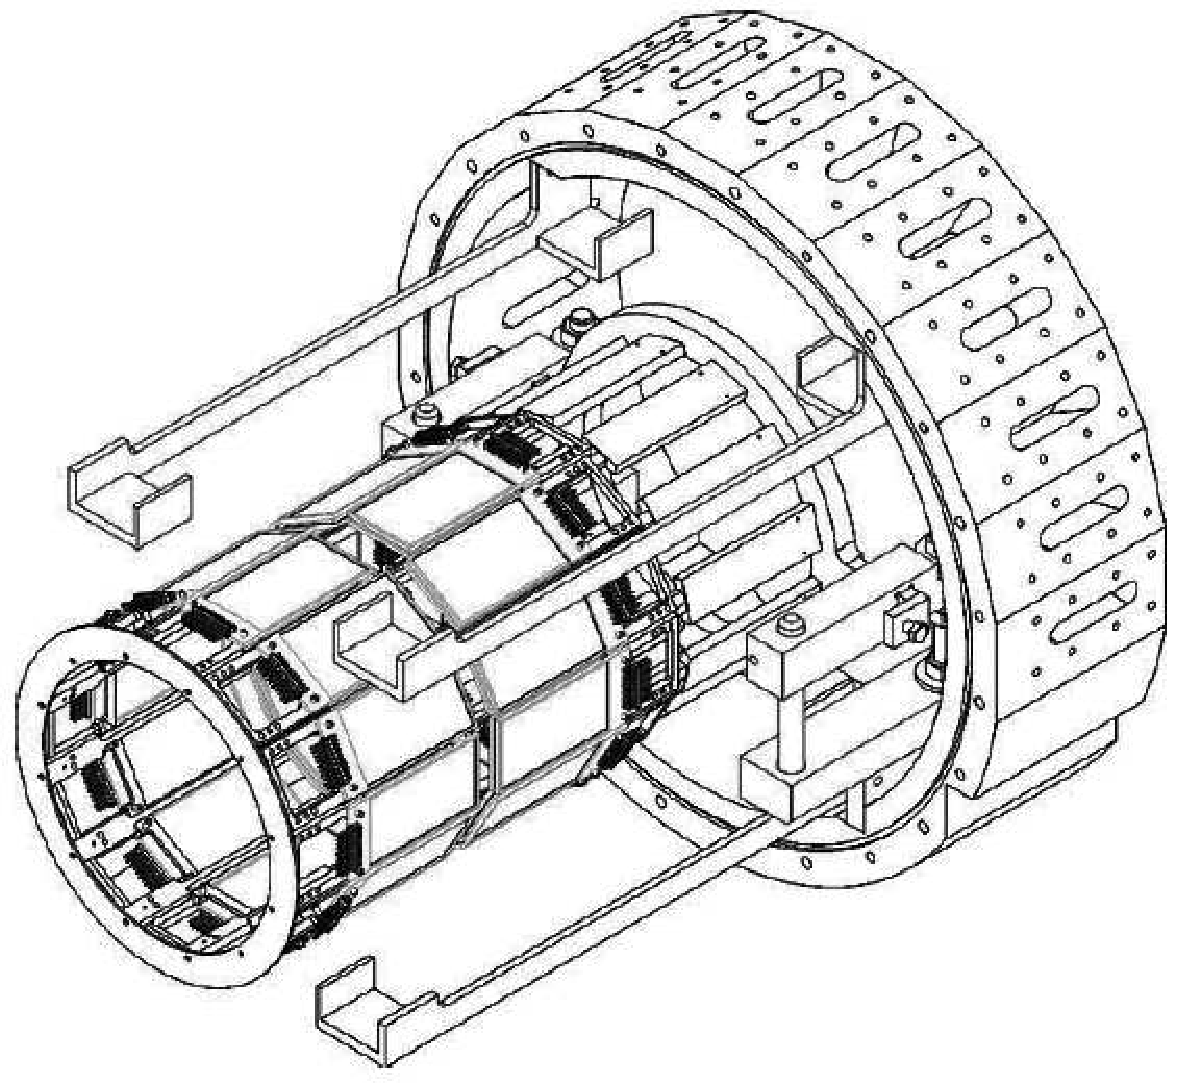
\includegraphics[width=\columnwidth,height=0.33\textheight,keepaspectratio]{Pain_2007-fig2}%
\caption[Engineering schematic of the ORRUBA detector system]{Engineering schematic of the ORRUBA detector system.  Beam enters from left.  In addition to showing two rings of detectors separated by a small gap, this figure also includes cable trays, the detector support structure and the preamplifier feedthrough ring.  Figure enhanced from Ref.~\cite{Pain_2007}.}%
\label{orruba}%
\end{figure}

The ORRUBA detector array, shown in Fig.~\ref{orruba}, is specifically designed to meet the challenges of measuring inverse kinematics: it has a large spacial coverage and is capable of making high resolution measurements of both energy and angle.  The details of the detector array construction are discussed in Ref.~\cite{Pain_2007}.  The ORRUBA detector array essentially consists of two rings of detectors positioned forwards and  backwards of $\theta_\mathrm{lab}=90^\circ$.  For the d($^{132}$Sn,p)$^{133}$Sn measurement, the upstream ring of detectors consisted of single-layer position sensitive detectors; the downstream ring was made up of $\Delta E$-$E$ telescopes, with the residual $E$ detectors also being position sensitive.  In this configuration, the detector array provides angular resolution of $<0.5^\circ$, position resolution of 0.5\,mm~FWHM, and (intrinsic) energy resolution of $<60$\,keV~FWHM.  Fig.~\ref{133Sn_e_spec_sim} shows a simulated spectrum of the d($^{132}$Sn,p)$^{133}$Sn based on these parameters.  The results of the simulation are in agreement with the analytic calculations of Fig.~\ref{sn-plots}.

\begin{figure*}
\begin{center}
\centering
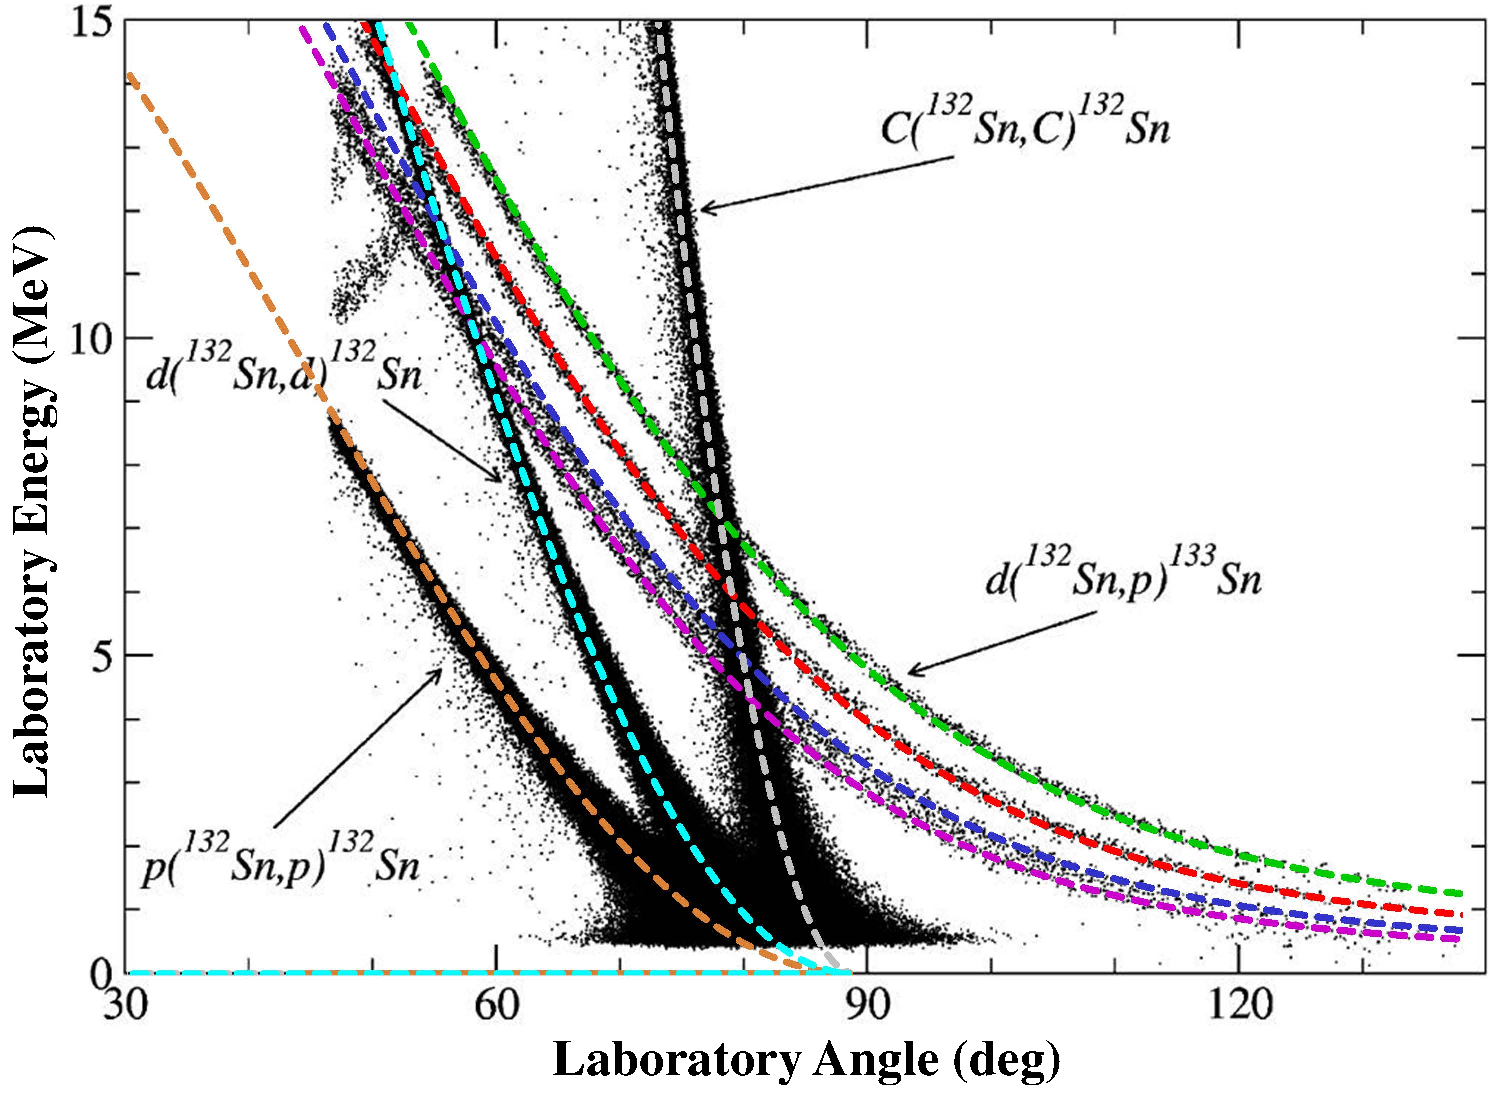
\includegraphics[keepaspectratio,height=0.3\textheight]{Pain_2007-fig1an-6}
\end{center}
\caption[Simulated $E_\mathrm{lab}$ vs. $\theta_\mathrm{lab}$ spectrum for the $d$($^{132}$Sn,$p$)$^{133}$Sn  reaction at 4.78\,\AMeV with ORRUBA]{(color online) Simulated $E_\mathrm{lab}$ vs. $\theta_\mathrm{lab}$ spectrum for the $d$($^{132}$Sn,$p$)$^{133}$Sn reaction at 4.78\,\AMeV with ORRUBA. The simulation includes elastic scattering of protons, deuterons, and $^{12}$C.  Analytical calculations have been plotted over the simulated results using the axes of the original figure.  The calculations are color-coded to match Fig.~\ref{133Sn_e}.  At $\theta_\mathrm{lab}=120^\circ$ 
  ($\theta_\mathrm{cm}=22.9^\circ$) the kinematic compression coefficient  is $\Delta E_\mathrm{lab}/\Delta E_\mathrm{cm}=0.34$.  Annotated    figure taken from Ref.~\cite{Pain_2007}.}
\label{133Sn_e_spec_sim}%
\end{figure*}

\subsection{Results}
\label{orrubaresults}
The ground-state and three excited states at $E_x=0.845$, 1.363, and 2005\,MeV were identified in this measurement. The state at $E_x=1.363\pm0.031$\,MeV was previously unobserved.  The $E_\mathrm{lab}$ versus $\theta_\mathrm{lab}$ proton spectrum produced is shown in Fig.~\ref{133Sn_e_spec}.  The analytic calculations of Fig.~\ref{sn-plots} have been plotted over the data (with re-calculated excitation energies).  Table~\ref{error_prop} shows that, neglecting target thickness effects, the $Q$-value resolution should be, at best, 133\,keV~FWHM.  Fig.~\ref{133Sn_e} shows the measured $Q$-value spectrum which has an energy resolution of over 300\,keV~FWHM.  Angular distributions were measured for the two lowest levels.  The ground state showed $\ell_n=3$ character, consistent with the $2f_{7/2}$ assignment; and the first-excited state at $E_x=0.845$ had an angular distribution characteristic of an $\ell_n=1$ transfer, corresponding to the $3p_{3/2}$ orbital.

\begin{figure*}
\begin{center}
\centering
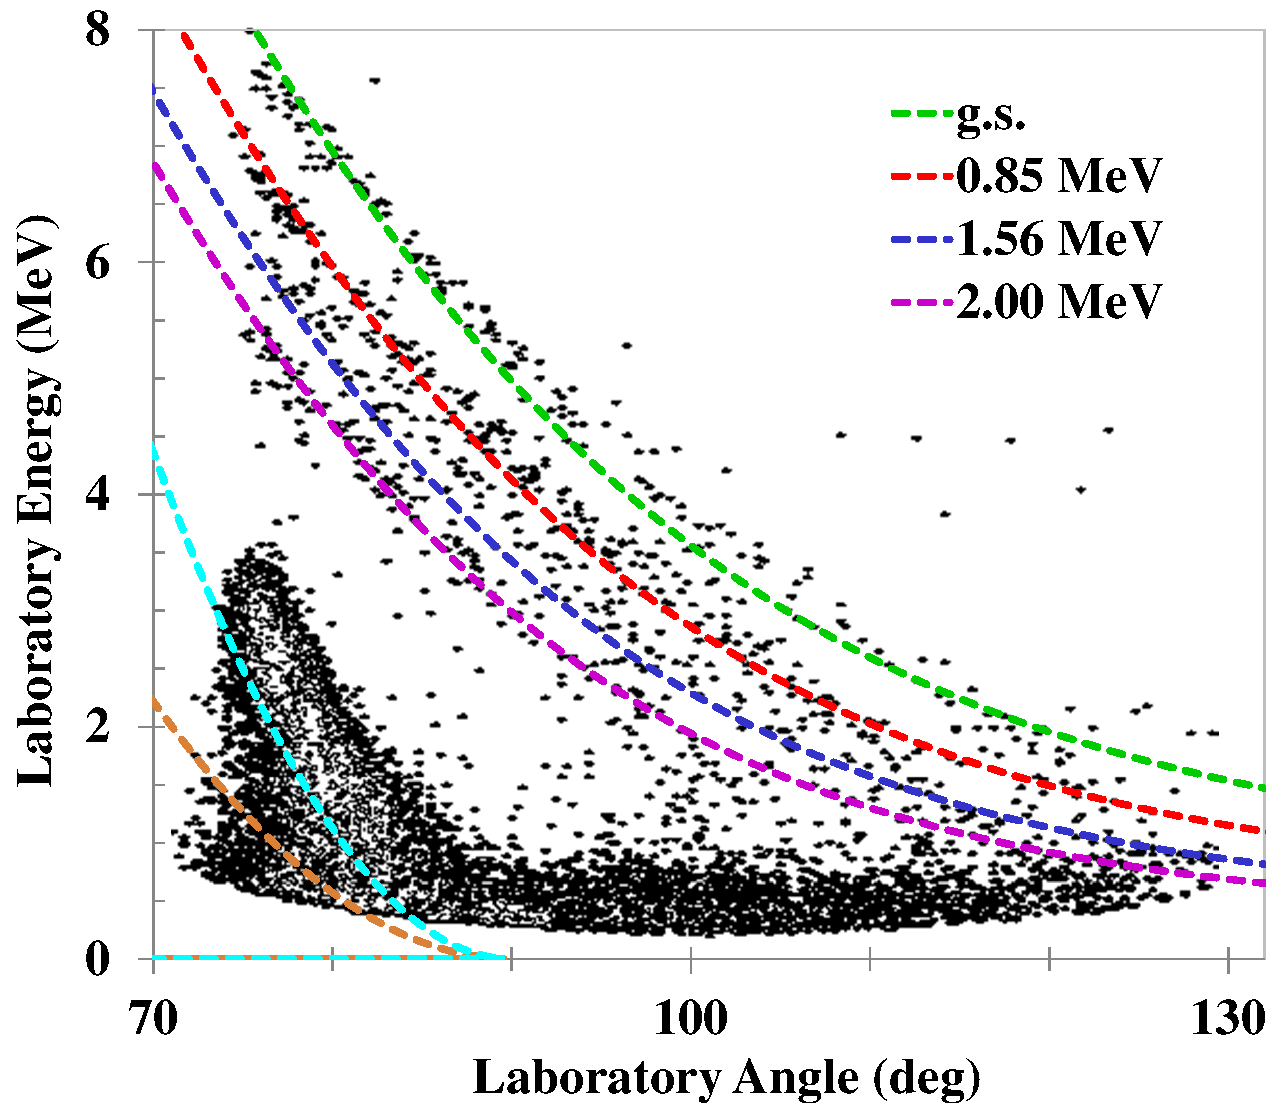
\includegraphics[keepaspectratio,height=0.3\textheight]{Jones_2007-2b}
\end{center}
\caption[Measured $E_\mathrm{lab}$ vs. $\theta_\mathrm{lab}$ spectrum for the $d$($^{132}$Sn,$p$)$^{133}$Sn reaction at 4.78\,\AMeV with ORRUBA]{(color online) Measured $E_\mathrm{lab}$ vs. $\theta_\mathrm{lab}$ spectrum for the $d$($^{132}$Sn,$p$)$^{133}$Sn reaction at 4.78\,\AMeV with ORRUBA.   Analytical calculations have been (roughly) plotted over the results, showing good agreement.  The axes of the calculations plot are shown.  Annotated figure taken from Ref.~\cite{Jones_2007}.}%
\label{133Sn_e_spec}%
\end{figure*}
%\subsection{Discussion}
Other reports are available in the literature of neutron transfer reactions in the $A=130$ region using ORRUBA.  An early proof-of-concept experiment was carried out using the lampshade SIDAR array and a prototypical form of the ORRUBA array to study the $^{124}$Sn($d$,$p$) reaction in inverse kinematics~\cite{Jones_2004}.  This measurement had a reported $Q$-value resolution of 200\,keV~FWHM.  %Using this set-up, the study was successful in producing a center-of-mass energy spectrum and the associated angular distributions.  Since then, 
Additional ($d$,$p$) studies have been carried out using %a more-complete form of 
the ORRUBA detector and other neutron-rich isotopes---$^{131}$Sn~\cite{Kozub_2008} and $^{134}$Te~\cite{Pain_2008}---both have excitation energy spectra with resolution on the order of 200--300\,keV~FWHM.  This collection of results provide a consistent description of the performance characteristics of this detector array.  In order to improve on the results obtained with ORRUBA, a detector system is needed which can avoid or suppress the effects of resolution degradation due to the covariance of measured quantities (kinematic broadening).

\begin{figure}[hb!]
\begin{center}
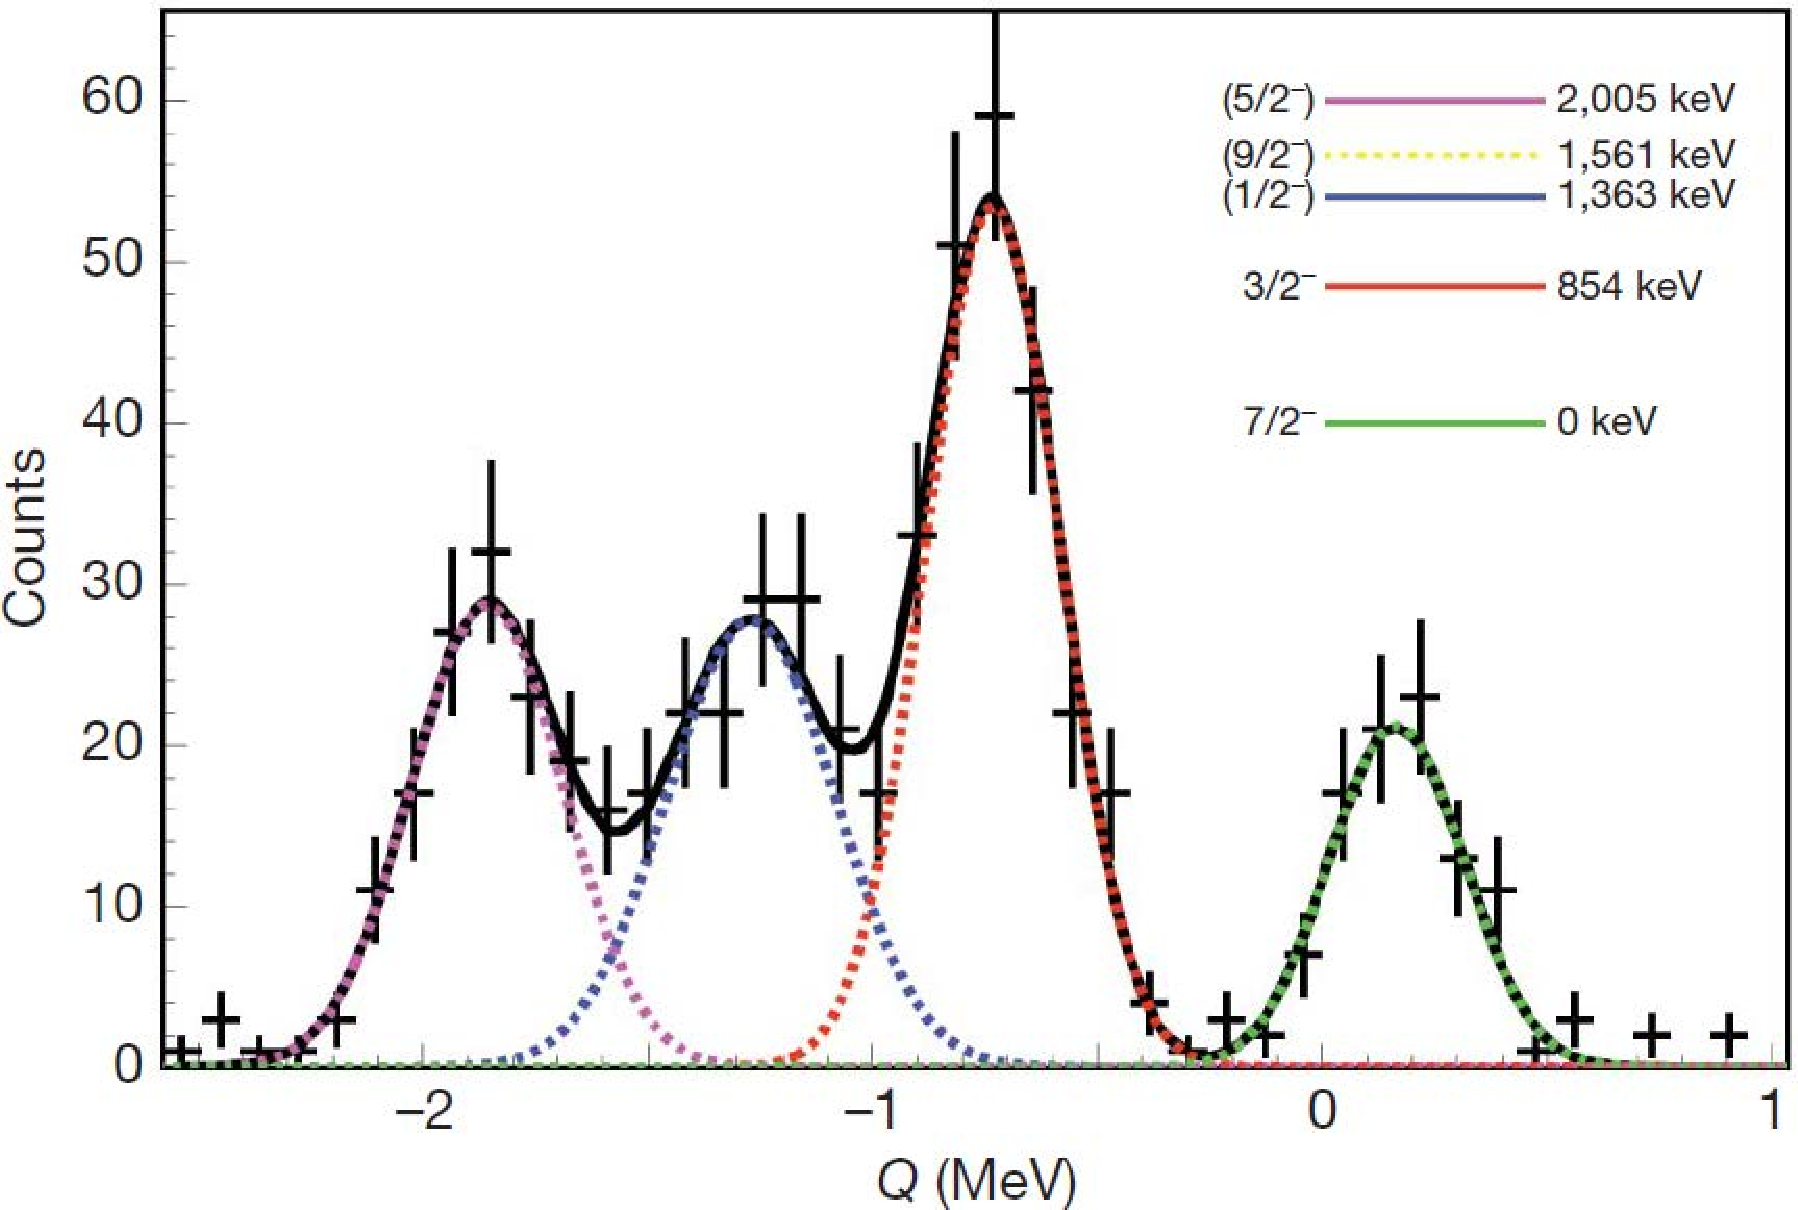
\includegraphics[keepaspectratio,width=\columnwidth,height=0.3\textheight]{Jones_2010-fig2-j}
\end{center}
\caption[$Q$-value spectrum from the $d$($^{132}$Sn,$p$)$^{133}$Sn reaction at 4.78\,\AMeV with ORRUBA]{(color online) $Q$-value spectrum from the $d$($^{132}$Sn,$p$)$^{133}$Sn reaction at 4.78\,\AMeV with ORRUBA.  Measured at $\theta_\mathrm{cm}=54^\circ$.  The $Q$-value resolution is 300\,keV~FWHM.  Figure taken from Ref.~\cite{Jones_2010}.}%
\label{133Sn_e}%
\end{figure}